\section{Prototipo 2.1: Generador de Registros Artificiales (GRA)}
En la sección actual se encuentran las modificaciones y/o agregaciones que se hicieron al Generador de Registros Artificiales.\\

\subsection{Modificaciones realizadas}
\begin{itemize}
\item Se agregó el caso de uso \textbf{CUGRA11: Agregar compras a clientes}.
\item Se agregó el caso de uso \textbf{CUGRA12: Agregar logros y nivel a clientes}.
\end{itemize}


\subsection{Análisis}


%%%%%%%%%%%%%%%%%%%%%%%%%%%%%%%%%%%%%%%%%%%%%%%%%%%%%%%%%%%%%%%%%%%
\title{\textbf{Diagrama de casos de uso}\\}
En la figura \ref{image:casosusoGRA11W} se muestra el diagrama de casos de uso del módulo Generador de Registros Artificiales.

\FloatBarrier
\begin{figure}[htbp!]
		\centering
			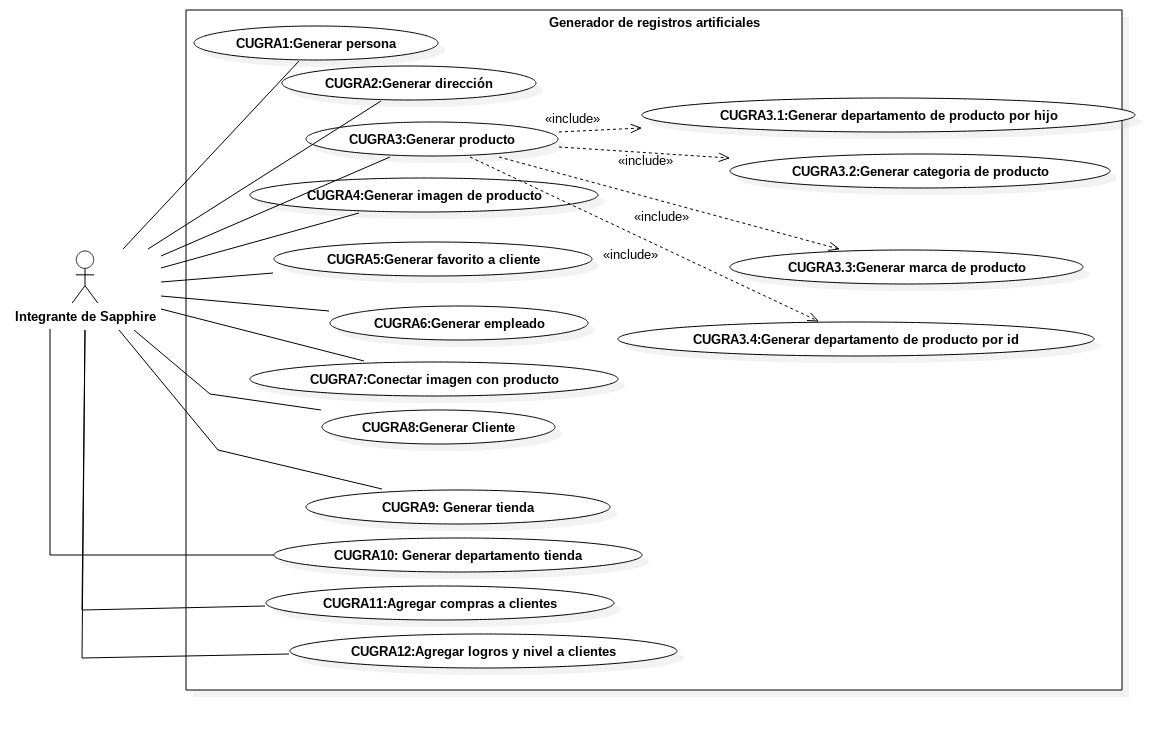
\includegraphics[width=1 \textwidth]{imagenes/CU/generadorRegistros11}
		\caption{Diagrama de casos de uso módulo Generador de Registros Artificiales.}
		\label{image:casosusoGRA11W}
\end{figure}
\FloatBarrier

\title{\textbf{Diagrama de clases}\\}
La descripción de los elementos en el diagrama de clases (figura \ref{image:diagramaclasesGRA11}) es la siguiente: 

\begin{itemize}
\item \textbf{Generator}: Clase encargada de la interacción con el usuario, muestra el menú y lee la opción ingresada por el usuario.
\item \textbf{FakerGenerator}: Clase engargada de tener la lógica para generar los registros artificiales.
\item \textbf{MysqlConnection}: Clase encargada de manejar la comunicación entre el módulo GRA y el gestor de base de datos MySQL.
\item \textbf{PsqlConnection}: Clase encargada de manejar la comunicación entre el módulo GRA y el gestor de base de datos PostgreSQL.
\end{itemize}

\FloatBarrier
\begin{figure}[htbp!]
		\centering
			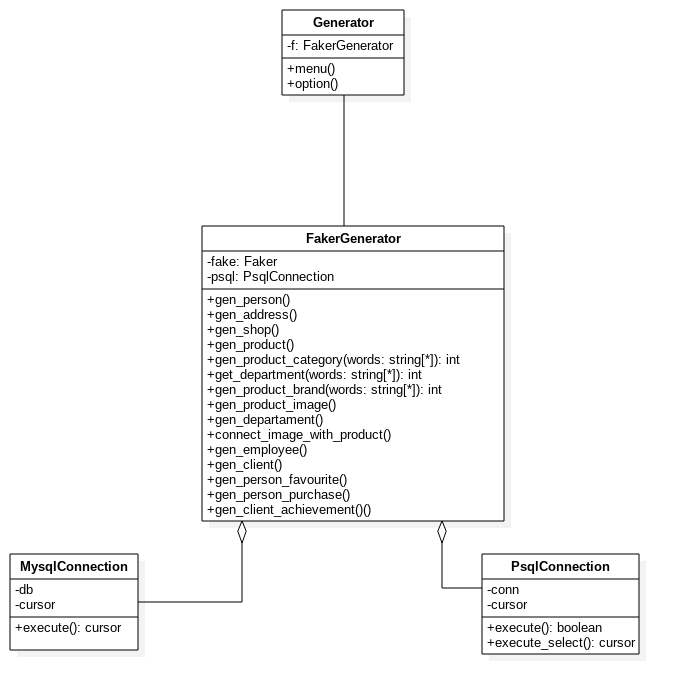
\includegraphics[width=.7 \textwidth]{imagenes/ClasesRuben/generador11}
		\caption{Diagrama de clases de módulo Generador de Registros Artificiales.}
		\label{image:diagramaclasesGRA11}
\end{figure}
\FloatBarrier

\subsection{Diseño}

\title{\textbf{Diagramas de secuencia\\}}
Durante este apartado se realizará una pequeña explicación de cada método agregado en este prototipo dentro de la clase FakerGenerator, además, dentro del mismo se muestran los diagramas de secuencia de dichos métodos separados dentro de sus respectivos apartados. \\

\title{\textbf{Agregar compras a clientes\\}}
Método encargado de cubrir el requerimiento funcional \textbf{RFGRA12} que permite realizar el registro de compras ficticias en el repositorio de datos. En la figura \ref{image:DSgenerarCompra} se muestra su diagrama de secuencia. 
\FloatBarrier
\begin{figure}[htbp!]
		\centering
			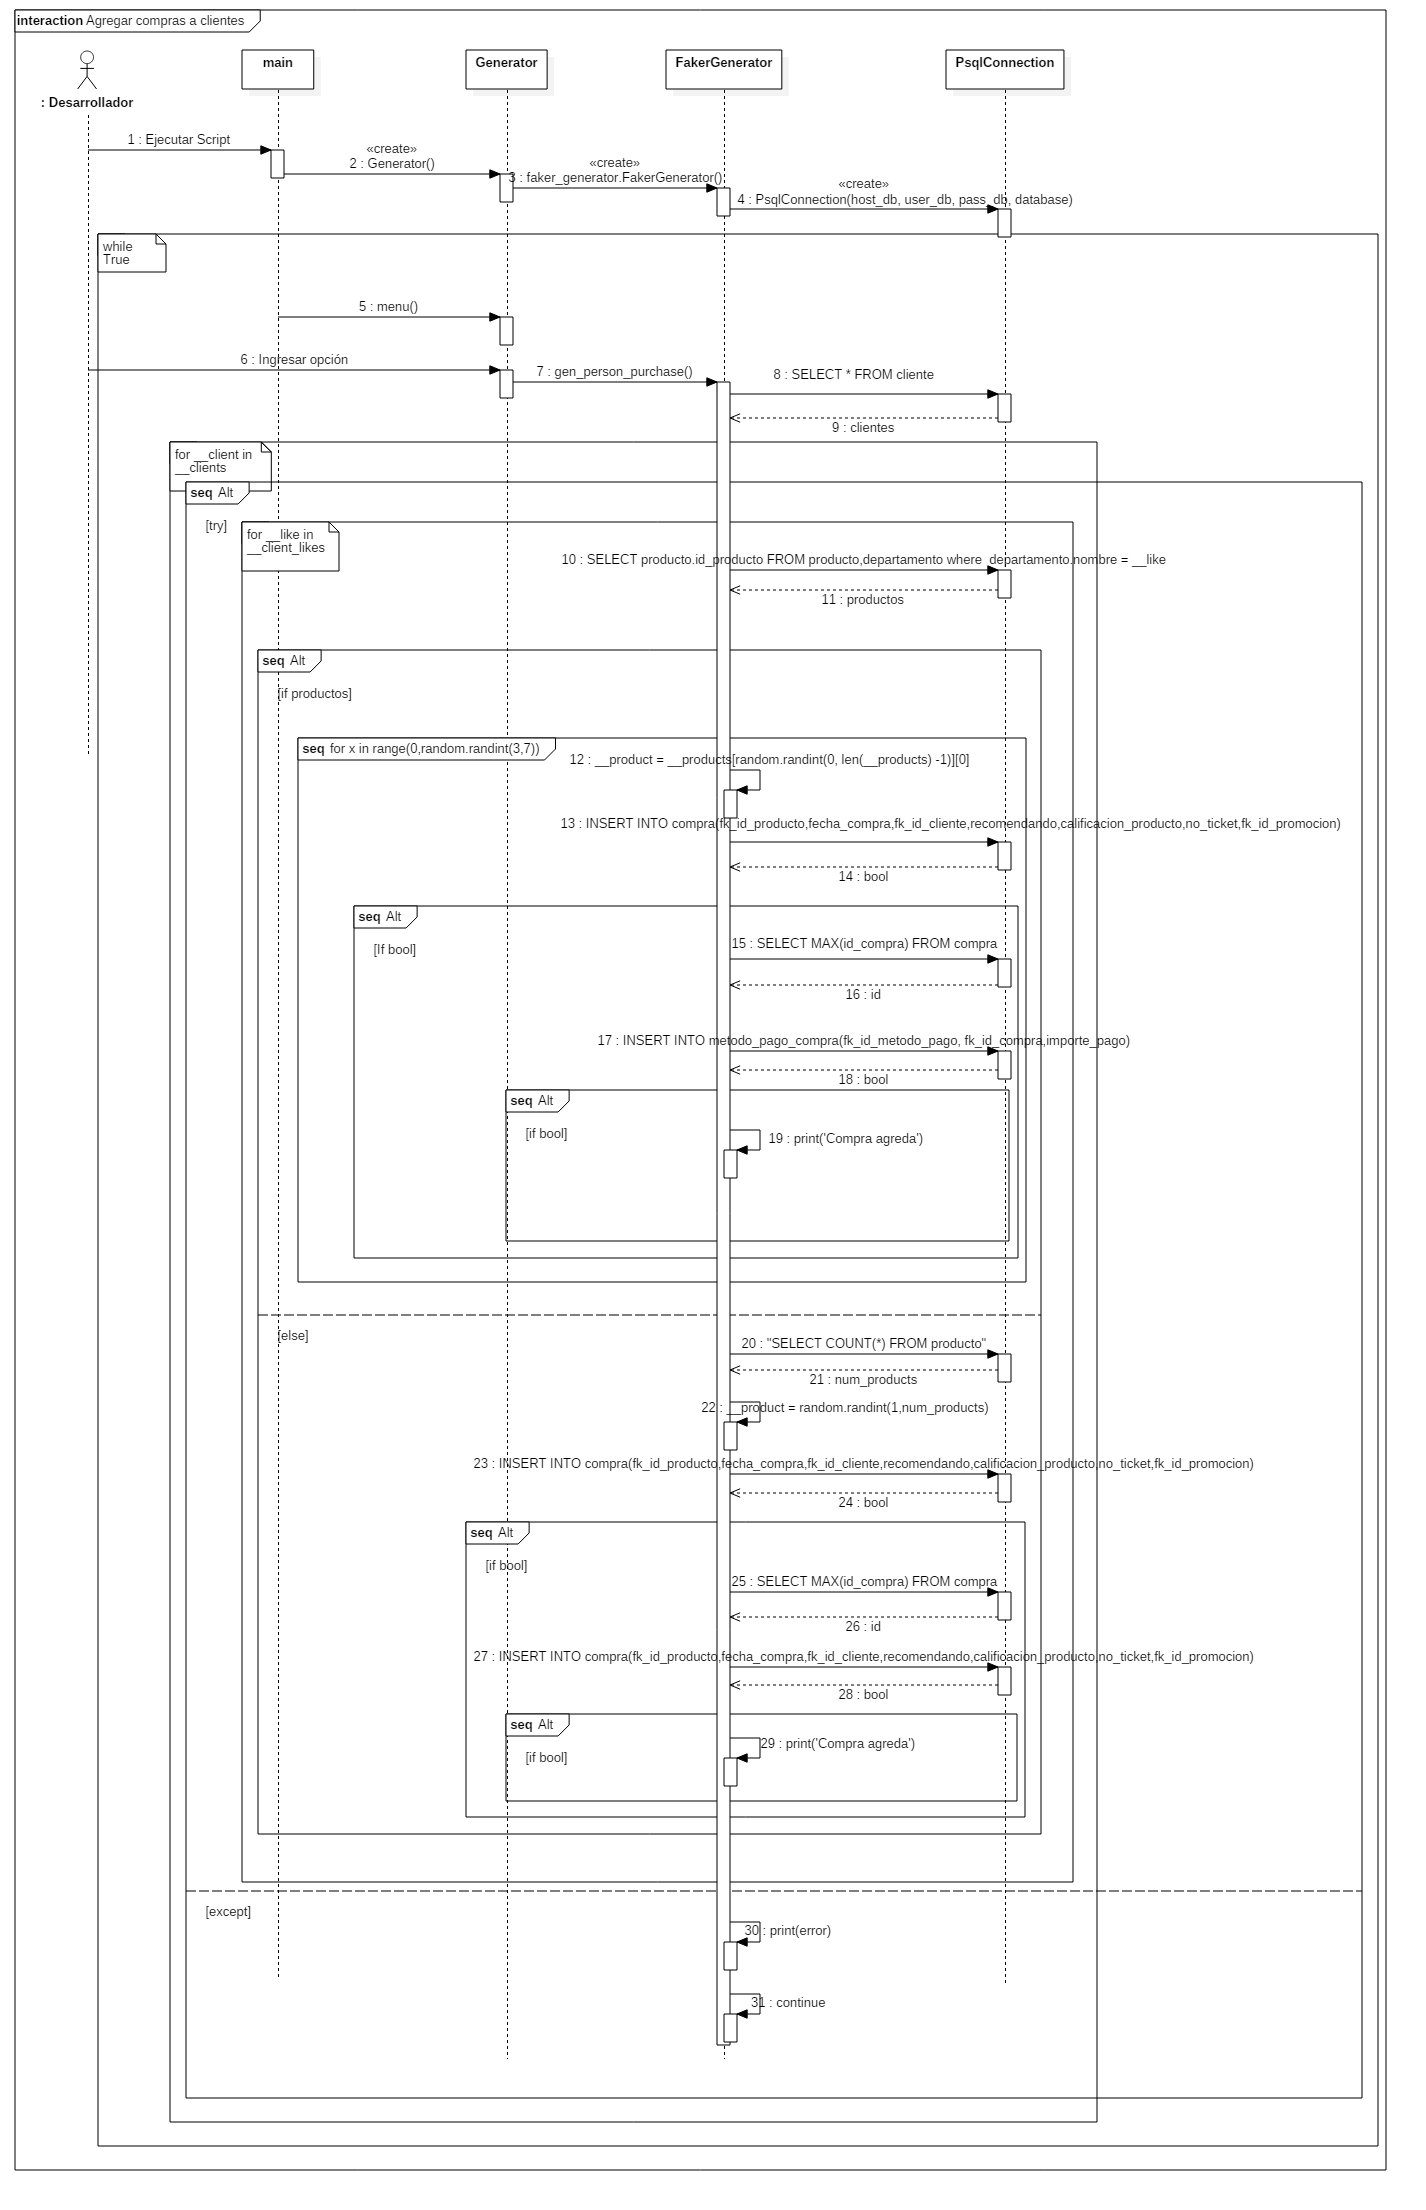
\includegraphics[width=.83 \textwidth]{imagenes/DSRuben/comprasproductos}
		\caption{Diagrama de secuencia para generar compras a clientes.}
		\label{image:DSgenerarCompra}
\end{figure}
\FloatBarrier

\title{\textbf{Asignar logros y nivel a clientes\\}}
Método encargado de cubrir el requerimiento funcional \textbf{RFGRA13} que actualiza los logros y el nivel de los clientes. En la figura \ref{image:DSnivel} se muestra su diagrama de secuencia. 
\FloatBarrier
\begin{figure}[htbp!]
		\centering
			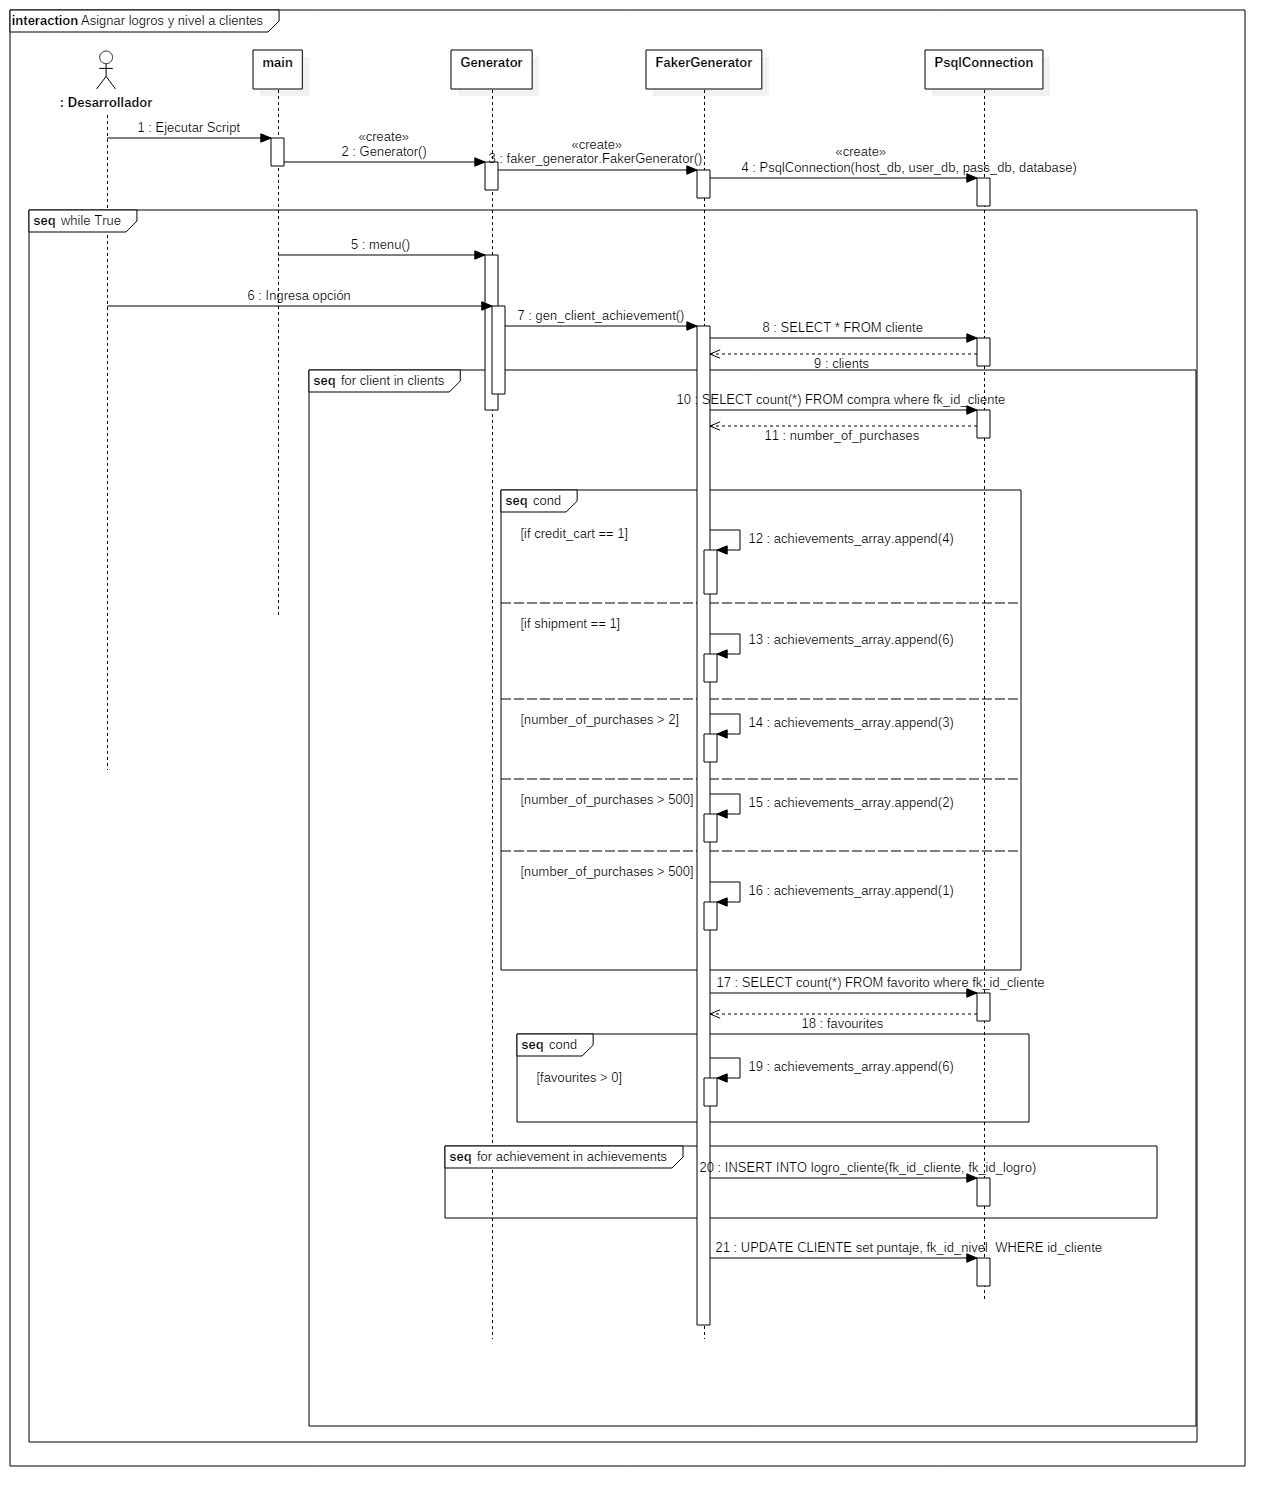
\includegraphics[width=1 \textwidth]{imagenes/DSRuben/gen_client_achievement}
		\caption{Diagrama de secuencia para asignar logros y nivel a clientes.}
		\label{image:DSnivel}
\end{figure}
\FloatBarrier

Finalmente la figura \ref{RA:11} muestra el menú del Generador de Registros Artificiales actualizado.

\FloatBarrier
\begin{figure}[htbp!]
		\centering
			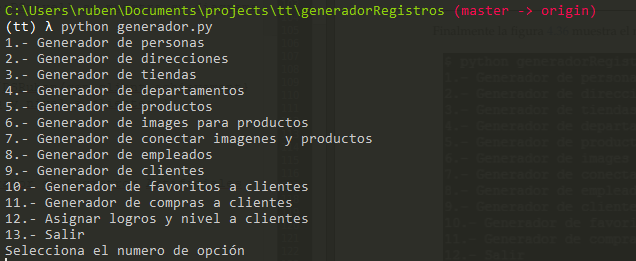
\includegraphics[width=.9 \textwidth]{imagenes/registrosArt/Menu11}
		\caption{UIRA: Menú}
		\label{RA:11}
\end{figure}
\FloatBarrier 